שידוך בגרף לא מכוון
$G = (V, E)$
הוא תת קבוצה בלתי תלויה של קשתות 
$M \subseteq E$.
כלומר, לכל שתי קשתות 
$e_1, e_2 \in M$
מתקיים ש-%
$e_1 \cap e_2 = \emptyset$.

\begin{definition}[שידוך מושלם]
שידוך יקרא מושלם אם 
$|M| = \frac{|V|}{2}$.
\end{definition}

\textbf{שידוך בגרף דו צדדי:}

בהינתן גרף דו צדדי,
$G = (L, R, E)$
נגדיר את רשת הזרימה,
$N = (G', c)$
כאשר
$$
\begin{array}{ll}
G' = (L \cup R \cup \{s, t\}, E')
\\
E' = \{uv : uv \in E, u \in L, v \in R\} \cup \{s\} \times L \cup R \times \{t\}
\\
c(e) = 1 & \forall e \in E'
\end{array}
$$

\textbf{דוגמה:}

\begin{center}
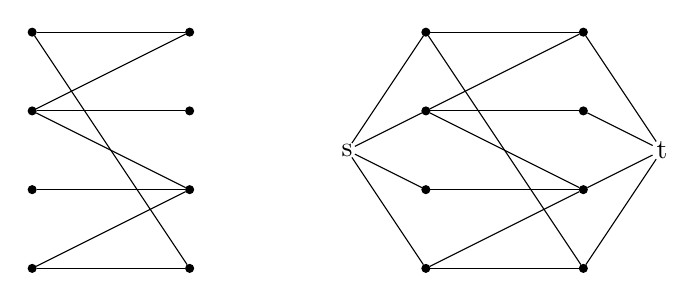
\begin{tikzpicture}[every node/.style={
	circle
	,draw
	,fill=black
	,inner sep=0
	,minimum size=1mm
}]

\foreach \i in {1,...,4}{
	\node(l\i) at(0,\i) {};
	\node(r\i) at(2,\i) {};
}

\foreach \u \v in {
	l1/r1,l1/r2%
	,l2/r2%
	,l3/r2,l3/r3,l3/r4%
	,l4/r1,l4/r4%
}{
	\draw[-] (\u) -- (\v);
}

\begin{scope}[xshift=5cm]

\node[fill=none, draw=none](s) at(-1, 2.5) {s};
\node[fill=none, draw=none](t) at(3, 2.5) {t};
\foreach \i in {1,...,4}{
	\node(l\i) at(0,\i) {};
	\node(r\i) at(2,\i) {};
	\draw (s) -- (l\i);
	\draw (r\i) -- (t);	
}

\foreach \u \v in {
	l1/r1,l1/r2%
	,l2/r2%
	,l3/r2,l3/r3,l3/r4%
	,l4/r1,l4/r4%
}{
	\draw[] (\u) -- (\v);
}
\end{scope}

\end{tikzpicture}
\end{center}


\begin{claim}
אם $M$ שידוך ב-$G$ אז קיימת זרימה $f$ ב-$N$ כך ש-%
$|f| = |M|$.

\begin{proof}
לכל 
$uv \in M$
נציב
$f(su) = f(uv) = f(vt) = 1$
ולכל שאר הקשתות נציב זרימה 0.
קל לוודא שזו אכן פונקציית זרימה עם ערך 
$|M|$.
\end{proof}
\end{claim}

\begin{claim}
אם $f$ זרימה בשלמים ב-%
$N$
אז קיים שידוך, $M$, ב-$G$ כך ש-%
$|M| = |f|$
\end{claim}

\begin{proof}
נגדיר
$M = \{uv : u \in L, v \in R, f(uv) = 1\}$.
קל לוודא שזהו אכן שידוך וש-%
$|M| = |f|$.
\end{proof}

\begin{corollary}
קיים אלגוריתם פולינומי שמוצא שידוך מקסימלי.
\end{corollary}

\begin{definition}[גרף רגולרי]
גרף לא מכוון יקרא $d$-רגולרי אם הדרגה של כל צומת היא $d$.
\end{definition}

\begin{claim}
לכל 
$d \geq 1$
בגרף דו צדדי $d$-רגולרי קיים שידוך מושלם.
\end{claim}

\begin{proof}
ראשית נשים לב שבגרף דו צדדי רגולרי מתקיים ש-%
$|L| = |R|$.
נסמן 
$|L| = n$
ומספיק להראות שקיימת זרימה (לאו דווקא שלמה) שערכה
$n$.

נגדיר:
$$
\begin{array}{ll}
f(sv) = 1 & \forall v \in L
\\
f(vt) = 1 & \forall v \in R
\\
f(uv) = \frac{1}{d} & \forall uv \in E : u \in L, v \in R
\end{array}
$$

אפשר לוודא שזו אכן זרימה עם ערך $n$.
\end{proof}
